
The algorithm developed in this thesis provides a way to combine two popular theories in machine learning - boosting and bagging. Both techniques provide a framework for ensemble learning and are meta-algorithms rather than learners. Rather than conducting the learning themselves, boosting and bagging are techniques that can be applied to rudimentary learners to achieve better performance. A learner can be defined as an algorithm with an underlying mathematical formulation to map input to output. A decision tree in the context of classification is an example of a learner. There are different ways to define meta-learning, I choose to define it in the following way. A meta-learner is a heuristic device that provides an architecture to learn from the output of learners (one or multiple). The algorithm proposed in section \ref{comb} of this chapter fits the definition of a meta learning system. In the next few sections I provide a short account of the primitive binary tree learner and a more detailed account of the boosting and bagging principles. The mathematical formulation of primitive tree learning is beyond the scope of this study.


\section{Tree learning}
\label{DT}

Decision trees (DT) are predictive and non-parametric models which use supervised learning for the task of classification. Given a set of training points $\{\textbf{x}_{i},y_{i}\}$ where $\textbf{x}_{i} \in \mathbb{R}^d$ is an input feature vector and $y_{i}$ is a categorical class variable the DT learns simple rules inferred from the input features with the goal of mapping them to their correct class labels.Typically, a decision tree has a top-down flow-chart like structure. 

At the top of the tree is a single \textit{source} node which at the beginning of the learning process has all the training data points. A tree starts learning by splitting the source node on the basis of a value test on a chosen input feature attribute. The value test essentially applies a threshold on the value of the chosen feature attribute and   partitions the training set. The partitions are expressed in the form of branches that emerge from the source node. This process is repeated in a recursive manner on each of the derived subsets. Fig \ref{flow_tree} illustrates the procedure of recursive partitioning. The choice of feature attribute to split on and the threshold for the value test are tied to user specified splitting criterion. The figure on the right shows the decision boundary that emerges as a result of applying univariate splits to the data. New data are classified on the basis of which rectangular region they fall into. In a high-dimensional feature space a decision tree gives hyper-rectangular regions. The tree in the figure has a depth of 4 and the nodes [A,$\ldots$,E] represent leaves, these might not be pure (i.e. contain samples of one class). The leaves are assigned a class based on the majority of samples that end up in that leaf.
 
\begin{figure*}
\hspace{-10mm}
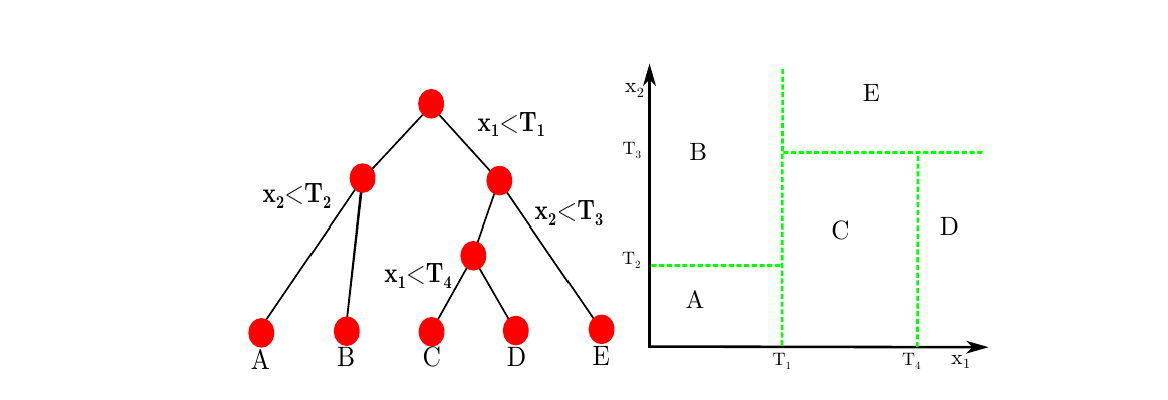
\includegraphics[scale=0.4]{images/tree_learner.png}
\caption{Tree learner. Adapted from \cite{treelearner}.}
\label{flow_tree}
\end{figure*}

The recursive phase of the tree continues until a stopping criterion is triggered. Some of the most common stopping rules are, 

\begin{enumerate}
\item{All of the training samples in a partition belong to the same class -- in this case, the node is converted to a leaf and recursion continues on the other branches.}
\item{User specified maximum depth has been reached.}
\item{A partition has less than the minimum number of samples required for a split, this parameter can be user specified, the default value is 2.}
\item{The best splitting criterion is not greater than a certain threshold.}
\end{enumerate} 

\section{Ensemble learning} 
\label{ensemble}

A single-pass classifier is a classifier that processes each event in the dataset once - the supervised training step is conducted by fitting a model to the whole dataset which is provided in the beginning with true labels. The decision tree introduced in the previous section is a classic example of a single pass classifier. This can be contrasted with ensemble classifiers that involve multiple iterations of training. In ensemble techniques training typically occurs through using a heterogeneous mix of classifiers or using copies of the same classifier initialized with different parameter settings. 

An example of an ensemble technique would be to train the dataset on a decision tree and a support vector machine and finally combine their predictions according to a certain weight to reach classification decisions. Ensembles can be built out of any diverse number of base learners. 

The ATLAS Higgs dataset is characterized by densely overlapping features (class overlap in the binary context was defined in chapter \ref{performance}). Popular published approaches that deal with the problem of class overlap suggest that the presence of highly overlaid classes significantly degrade the performance of single pass classifiers and point to the need for more sophisticated techniques like \textit{ensembles}. While ensemble techniques are known to be very effective in improving performance their main criticism is that techniques to combine different classifiers are not rooted in mathematical theory. The choice of base learners are guided by empiricism - characteristics of the data, bounds on model complexity, time and memory.

In the next sections we discuss two of the most popular themes in ensemble learning - boosting and bagging.  

\section{Boosting: concept \texorpdfstring{$\&$}{} description}

The aim of this section is to present the concept of boosting and describe one of the most fundamental expressions of the idea - the AdaBoost algorithm \cite{scapire} won the 2003 G$\ddot{o}$del prize. 

The success of boosting techniques is attributed to the way they tackle the problem of class overlap. Boosting works by iteratively training `weak' learners to build a master learner which is significantly better at the task. The decision rule for the master learner is a weighted combination of the weak learners outcomes and the weights are usually a function of the weak learners accuracy. A weak learner is a classifier that can classify samples better than random guessing.

Boosting ensures that samples in the most ambiguous regions of the feature space which are repeatedly misclassified are encountered in multiple stages of the training process, thereby allowing the classifier to focus on the hard to classify events. This explains how boosting achieves low bias. At each iteration it improves accuracy by classifying few more points than in the previous stage correctly without disrupting the correct classifications from previous stages. 

While boosting is considered to be one of the best off-the-shelf classifiers in the world it is prone to overfitting the training data. This makes it a high variance classifier. Boosting with several stages of tree learning can rapidly overfit as trees are low bias high variance learners. To control over-fitting while using boosting is one of the main challenges in using this technique. Boosted decision trees (BDTs) use decision trees (or decision stumps - a one-level decision tree) as base learners within the context of boosting and have been the benchmark algorithm for multivariate analysis and classification problems for particle identification at CERN. 

\subsection{AdaBoost}

AdaBoost is a meta-algorithm which uses the principle of boosting. It has a cascade architecture that trains the data in multiples stages where each stage uses information from the output of the previous stage. AdaBoost initiates the first stage by assigning a uniform weight to each training sample. At the end of the first stage it increases the weight on the misclassified samples in a weight update step. This process is continued until the misclassification rate saturates. 

Consider a binary classification problem with input vectors $\mathbf{D} = \{(\mathbf{x}_{1},y_{1},w_{1}) \ldots (\mathbf{x}_{n},y_{n},w_{n})\}$ with binary class labels $y_{i} \in \{-1,+1\}, \forall i=1 \ldots n$. 

At the start of the algorithm, the training data weights $\{w_{i}\}$ are initialized to $w_{i}^{(1)} = 1/n, \forall i=1 \ldots n$. A base classifier $h_{1}(\mathbf{x}): \mathbf{D} \rightarrow \{-1,+1\} $ that misclassifies the least number of training samples is chosen. Formally, $h_{1}(\mathbf{x})$ minimizes the weighted error function given by, 

\begin{equation}
R(h_{1}) = \sum_{i=1}^{N}w_{i}\mathbf{I}(h_{1}(\mathbf{x}) \neq y_{i})
\end{equation}
where $\mathbf{I}$ is the indicator function.  
 
After the first round of classification,  the coefficient $\alpha_{1}$ is computed that indicates the confidence in the classifier. It is chosen to minimize an exponential error metric given by,

\begin{align*}
E &= \sum_{i=1}^{N}e^{y_{i}\alpha_{1}h_{1}(\mathbf{x}_{i})}\\
&= \sum_{y_{i}\neq h_{1}(\mathbf{x}_{i})}e^{\alpha_{1}} + \sum_{y_{i} = h_{1}(\mathbf{x}_{i})}e^{-\alpha_{1}}
\end{align*}

\begin{align*}
\frac{dE}{d\alpha_{1}} &=  \sum_{y_{i}\neq h_{1}(\mathbf{x}_{i})}e^{\alpha_{1}} - \sum_{y_{i} = h_{1}(\mathbf{x}_{i})}e^{-\alpha_{1}} \\
&\Rightarrow \sum_{y_{i}\neq h_{1}(\mathbf{x}_{i})}e^{\alpha_{1}} = \sum_{y_{i} = h_{1}(\mathbf{x}_{i})}e^{-\alpha_{i}}\\
&\Rightarrow (N - N_{c})e^{\alpha_{1}} = N_{c}\frac{1}{e^{\alpha_{1}}}   \\
&\textrm{where $N_{c}$ is number of correctly classified samples by $h_{1}$}\\
&\Rightarrow e^{2\alpha_{1}} = \frac{N_{c}}{N - N_{c}}\\
&\Rightarrow \alpha_{1} = \frac{1}{2}\ln\bigg(\frac{N_{c}}{N-N_{c}}\bigg)
\end{align*}

Denoting $\epsilon_{1} = \dfrac{N - N_{c}}{N}$ as the error rate for $h_{1}$,

\begin{align}
\alpha_{1} = \frac{1}{2}\ln\bigg(\frac{1-\epsilon_{1}}{\epsilon_{1}}\bigg)
\label{alphas}
\end{align}

The weight update equation at each stage is given by, 

\begin{align*}
w_{i}^{(m+1)} = w_{i}^{(m)}e^{\alpha_{m}\mathbf{I}(h_{m}(\mathbf{x}_{i}) \neq y_{i})}
\end{align*}

The master learner $M_{h}(\mathbf{x})$ for a $M$ stage classifier is given by,

\begin{equation}
M_{h}(\mathbf{x}) = \sign\bigg( \sum_{m=1}^{M}\alpha_{m}h_{m}(\mathbf{x})\bigg)
\label{master}
\end{equation}
 
The intuitive idea behind AdaBoost is that by increasing the weights on misclassified samples successively, the classifier places greater emphasis on samples that are hard to classify. Traditional choices for weak learners in AdaBoost are logistic regression, decision stumps, decision trees and naive bayes classifiers. 

\begin{figure}[ht]
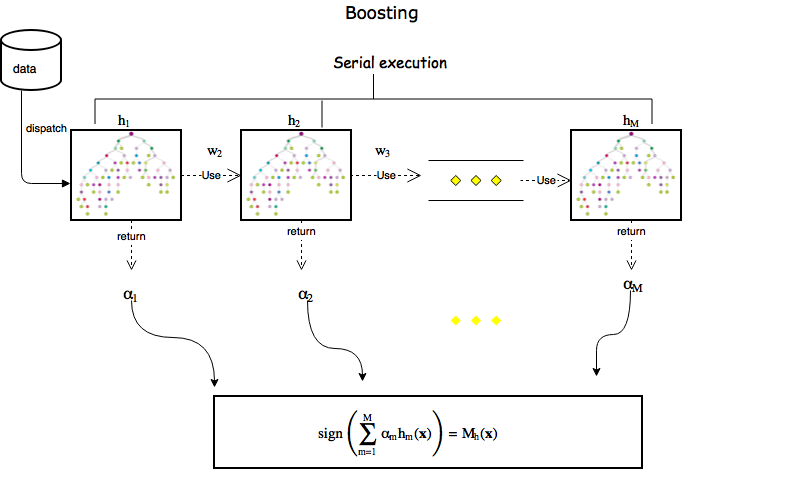
\includegraphics[width=\textwidth]{images/boostingflow.png}
\label{boosting}
\caption{Data Flow in boosting with single trees. In each iteration the weights $w_{i}$ are updated to focus more on the events misclassified in the previous stages. The $\alpha_{i}$s are the learning rates which are tied to performance of each base learner.}
\end{figure}

\section{Bagging: concept \texorpdfstring{$\&$}{} description}

Bagging derives from the words \textbf{b}ootstrap \textbf{agg}regat\textbf{ing} and was a technique popularised by Leo Brieman who first published the idea in 1996 \cite{bagging}. The bagging technique helps stabilise classifiers by training a single classifier on multiple bootstrap samples of the training data set. We end up with multiple versions of the same classifier which only differ in their training sets. A bootstrap sample is a result of drawing a uniform random sample \textbf{with replacement} from a dataset of size $n$. The size of the bootstrap usually is the same as the original dataset. Due to sampling with replacement a bootstrap sample most likely has repeated samples, this increases the predictive force of the base learner applied on those samples. Sampling sufficiently large number of times ensures that each element appears as duplicates in atleast one of the bootstrap samples.

Bagging can improve accuracy and is most useful when applied to unstable and high variance base learners, like decision trees. The instability of the base learner is the key requirement. 

Brieman notes:

``\textit{The vital element is the instability of the prediction method. If perturbing the learning set can cause significant changes in the predictor constructed, then bagging can improve accuracy.}"

Gains from bagging cannot be realized for classifiers which are stable and deterministic. Procedures like $k$-nearest neighbour are stable as they predict results based on a fixed spatial distribution of the training data. %Unstable classifiers have an element of randomization embedded in them, for instance, trees in their construction consider a random subset of features to select the best split from at each node. Hence, training a decision tree on a perturbed training dataset leads to different results \cite{bagging}. 
   
Given a training dataset $\mathbf{D} = \{(\mathbf{x}_{1},y_{1},w_{1}) \ldots (\mathbf{x}_{n},y_{n},w_{n})\}$ with binary class labels $y_{i} \in \{-1,+1\}$ and $w_{i} \in \mathbb{R}$  . Let $t: \mathbf{D} \rightarrow \{-1,+1\}$ be the decision tree learner that assigns an input vector $\mathbf{x}_{i}$ to a predicted label $\hat{y}_{i}$ and $\{\mathbf{D}^{(b)}\}$ be the sequence of bootstrap samples taken from $\mathbf{D}$. Each input $\mathbf{x}_{i}$ may appear in repeated bootstraps $\{\mathbf{D}^{(b)}\}$ or in none at all. The aggregated forest $t_{agg}$ is an expectation over individual trees $E(t)$. If $t$ predict a class label $\{-1,+1\}$, then $t_{agg}$ aggregates through majority voting. If $t$ predicts a probability then, $t_{agg}$ uses an arithmetic average of probability estimates from individual tree outputs $t(\mathbf{x}_{i})$. The number of bootstrap samples to use in bagging is usually established through computing the out-of-bag \footnote{OOB error refers to the prediction error of each sample $\mathbf{x_{i}}$ using trees which did not choose $\mathbf{x_{i}}$ in the bootstrap.} (OOB) error and stopping at the point at which the OOB saturates. A bootstrap sample $\{\mathbf{D}^{(b)}\}$ of size $n$ from $D$ will contain approximately 63.2$\%$ unique samples. 

The probability of an arbitrary sample $\mathbf{x}_{i}$ not being picked in $n$ draws is $(1-1/n)^{n}$. The result then follows from ($1 - \lim_{n \rightarrow \infty}(1 - 1/n)^n) =  (1 - 1/e) \approx 0.632$.

\begin{figure}
\centering
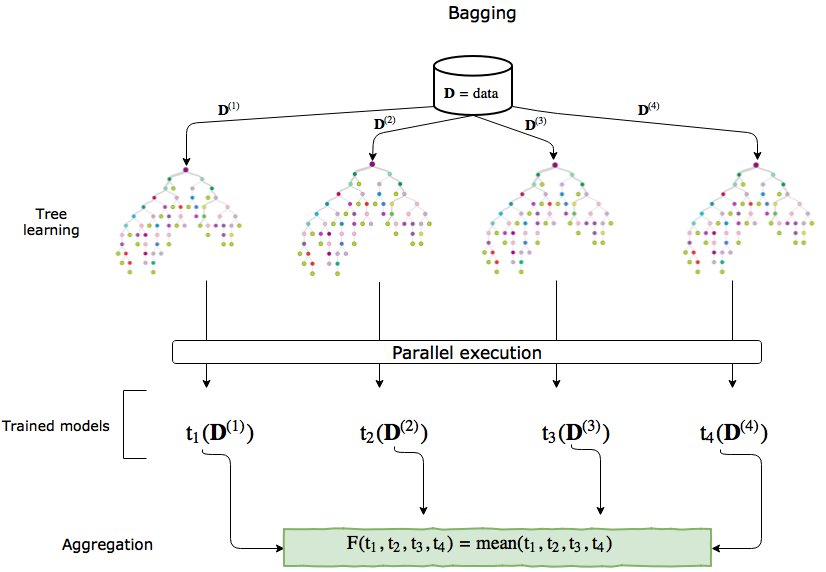
\includegraphics[width=\textwidth]{images/baggingflow.png}
\label{bagging}
\end{figure}

\subsection{Random Forest (RF)}

\gls{RF} is the trademark algorithm exemplifying bagging principle. A random forest as the name suggests is a collection of tree learners each trained on a bootstrap sample $\mathbf{D}^{(b)}$ of the training data $\mathbf{D}$. There are two sources of randomness in a random forest, the formation of bootstrap samples and the random selection of features considered at each node in the context of growing a single decision tree \cite{subspace}. The difference between the general bagging scheme for trees and a random forest is the second source of randomness also called $feature$ bagging. Many times, if there are $s$ features $\sqrt{s}$ (rounded down) features are randomly picked for consideration at each node.

The performance of a random forest depends on the strength of individual trees in the forest and the correlation between them. Perturbing the training set $\mathbf{D}$ by introducing duplicates through bootstraps is one way of decorrelating the trees however more different trees can be constructed if a random subset of features is selected at each split. In high dimensional data with a large number of features, this expands the universe of possible trees that can be constructed and introduces more tree dissimilarity.

Overall, the only disadvantage random forests have relative to a single pass decision tree is the loss of interpretability of the forest structure. A single decision tree has the nice property of being fully interpretable, a tree is essentially a `white-box' model which can be de-constructed  compared to models like artificial neural networks where the input to output flow cannot be easily unwound.

\begin{algorithm}[h]
\caption{Random Forest with $M$ trees}
\begin{algorithmic}[1]
\STATE \textbf{Training}:
\STATE \textbf{Input}: Training set $\mathbf{D}$, tree learner $t$ 
\STATE \textbf{Output}: Forest of trees $F(t_{1} \ldots t_{M})$ 
\item[]
\FORALL{$b$ = 1 \ldots $M$}
\STATE  \textbf{Construct} a bootstrap sample ${D^{(b)}}$ (sample uniformly with replacement from $\mathbf{D}$)
\STATE \textbf{Fit} tree learner $t_{b}$ on sample $D^{(b)}$
\ENDFOR
\RETURN $F(t_{1} \ldots t_{M})$  
\item[]
\STATE \textbf{Testing}:
\STATE \textbf{Input}: Test set $\mathbf{L} = \{\mathbf{x}_{i}\}_{i=1}^{n}$, forest of trees $F(t_{1} \ldots t_{M})$ 
\STATE \textbf{Output}: Predicted labels $\{\hat{y_{i}}\}_{i=1}^{n}$ 
\item[]
\FORALL {$\mathbf{x}_{i} \in \mathbf{L}$}
\STATE \textbf{Predict} $\hat{y}_{i} = F(\mathbf{x}_{i}) = F(t_{1}(x) \ldots t_{M}(x)) = E_{M}(t(\mathbf{x_{i}}))$
\ENDFOR
\RETURN $\{\hat{y_{i}}\}_{i=1}^{n}$
\end{algorithmic}
\label{rf}
\end{algorithm}

\section{Boosting vs. Bagging}

The meta techniques boosting and bagging specialize in two different aspects of the learning problem. The main focus in boosting is reducing bias and converging towards higher accuracy rates, it does so by narrowing focus on the hard to classify samples by repeatedly scaling up weights on these samples. While this gives powerful master learners, it is not resistant to the problem of over-fitting, which means that while they have the ability to fit very well to training data this needs to be balanced with their ability to generalize on unseen data. 

In bagging the main focus is variance reduction. A single unstable model is sensitive to noise in the training data and as a stand alone might fail to meet performance requirements however an average of several hundred unstable models which are uncorrelated is less sensitive to noise. A collection of trees trained on the same training dataset will give correlated results and the gains from averaging are subdued, however, a collection of trees each trained on a different training dataset gives de-correlated models. 

Boosting has no random elements, it goes from one stage of learning to the next and transfers an updated weight distribution which is fully determined by performance in the prior stage of learning. The weight distribution is adjusted to give misclassified samples more weight. The higher the weight the greater the influence of the sample on the learned model. Boosting is a closed form model, it only requires specification of the base learner and the number of stages of boosting. In contrast, bagging works because of the effectiveness of randomization. Randomization in creating bootstrap samples and feature subspace selection generate diversity in models and aggregating them helps overcome the instability of singular models. 

\section{Extremely Randomized Trees (ET)}

In the world of meta algorithms, bagging and boosting dominated the sphere for most of the nineties. There are several publications devoted to comparing the performance of each of the techniques on several classification datasets. \gls{ET} is one of the newer incarnations of the random forest method. The paper on ET was published in 2005 by  Geurts, Ernst and Wehenkel \cite{xrf}. The main principle is the introduction of randomization in the tree construction process. While random forests attempt to create diversified trees by using a bootstrap sample, ETs work like random forests but take the randomization one step further by choosing a random split point at each node rather than searching for the best split. This ensures the creation of strongly decorrelated trees. From the viewpoint of computational efficiency, ETs offer an advantage as they do not need to look for the most optimal split at each node. 

The random split generating algorithm from \cite{xrf} is summarized in \ref{randomsplits}. 

\begin{algorithm}[H]
\caption{Random Splitting algorithm}
\begin{algorithmic}[1]
\STATE \textbf{Input}: Training set $\mathbf{D}$
\STATE \textbf{Output}: A split $c_{j}$ which is a scalar value from a single feature vector of the training set $\mathbf{D}$  
\item[]
\STATE \textbf{Select} $K$ features ${a_{1}, \dots , a_{K}}$ at random from $\mathbf{D}$
\STATE \textbf{Select} $K$ splits $\{c_{1}, \dots , c_{K}\}$, one per feature for the $K$ features chosen in the previous step; each $c_{i}$ is selected at random from the range of the feature values $\forall i = 1, \dots K$  
\STATE Rank the splits $c_{i}$ by a criterion say $Q$ which gives a score $Q(\mathbf{D}, c_{i}) \in \mathbb{R}$ for each split. 
\STATE Select $c_{*} = max_{i=1 \dots K}Q(\mathbf{D}, c_{i})$  
\RETURN $c_{*}$
\end{algorithmic}
\label{randomsplits}
\end{algorithm}

A forest of extremely randomized trees trains each randomized tree on a bootstrap sample $\mathbf{D}^{(b)}$ and averages the output of randomized trees.
\begin{algorithm}[H]
\caption{Extremely Randomized $M$ trees}
\begin{algorithmic}[1]
\STATE \textbf{Training}:
\STATE \textbf{Input}: Training set $\mathbf{D}$, tree learner $t$ 
\STATE \textbf{Output}: Collection of extremely randomized trees $\{t_{1} \ldots t_{M}\}$
\item[]
\FORALL{$b$ = 1 \ldots $M$}
\STATE \textbf{Construct} a bootstrap sample ${D^{(b)}}$ (sample uniformly with replacement from $\mathbf{D}$)
\STATE \textbf{Fit} tree learner $t_{b}$ on sample $D^{(b)}$ using the Random Splitting Algorithm (see \ref{randomsplits})
\ENDFOR
\RETURN Collection of fitted trees $\{t_{1} \ldots t_{M}\}$  
\item[]
\STATE \textbf{Testing}:
\STATE \textbf{Input}: Test set $\mathbf{L} = \{\mathbf{x}_{i}\}_{i=1}^{n}$, collection of extremely random trees $\{t_{1} \ldots t_{M}\}$ 
\STATE \textbf{Output}: Predicted labels $\{\hat{y_{i}}\}_{i=1}^{n}$ 
\item[]
\FORALL {$\mathbf{x}_{i} \in \mathbf{L}$}
\STATE \textbf{Predict} $\hat{y}_{i} = agg(t_{1}(\mathbf{x_{i}}), \ldots, t_{M}(\mathbf{x_{i}}))$
\ENDFOR
\RETURN $\{\hat{y_{i}}\}_{i=1}^{n}$
\end{algorithmic}
\label{eforest}
\end{algorithm}

\section{Combining Bagging and Boosting} 
\label{comb}

There are several works which compare the effectiveness of bagging and boosting on several datasets. The consensus is that no technique is superior to the other and the effectiveness of the technique is tied to the characteristics of the problem at hand. For final testing on the Higgs dataset we propose an algorithm that is a variant of the boosted decision tree.  

The boosted ensemble works as a sequential learner but at each stage is supported by a bagged ensemble of primitive trees. There is very little to no evidence of models where bagging and boosting are harnessed together as such an ensemble is hard to optimize and not easily interpretable. We show that using extremely randomized trees as a base learner to boosting shows strong performance in the context presented by the classification task on the Higgs dataset. Simultaneously, we show that using a traditional random forest as a base learner to boosting does not prove to be very effective. The key trick here is the randomization introduced by extremely random trees proves to be effective in predicting more events accurately. We call these models - Boosted random forests (\gls{BRF}) and Boost extremely random trees (\gls{BXT}). The algorithms are tested on the $H \rightarrow \tau^{+} \tau^{-}$ binary classification task. The next chapter presents some results and useful insights, it also draws comparisons with the leading solutions to the problem. 

\begin{sidewaysfigure}
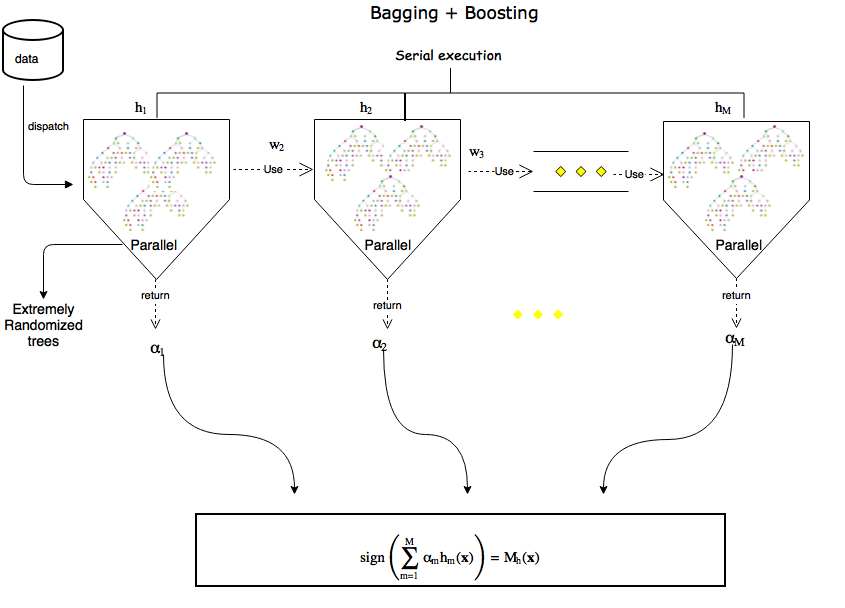
\includegraphics[scale=0.6]{images/bagboost.png}
\caption{Unified bagging + boosting algorithm using extremely random trees}
\end{sidewaysfigure}


